% Options for packages loaded elsewhere
\PassOptionsToPackage{unicode}{hyperref}
\PassOptionsToPackage{hyphens}{url}
\PassOptionsToPackage{dvipsnames,svgnames,x11names}{xcolor}
%
\documentclass[
  11pt,
  a4paperpaper,
]{scrreprt}

\usepackage{amsmath,amssymb}
\usepackage{iftex}
\ifPDFTeX
  \usepackage[T1]{fontenc}
  \usepackage[utf8]{inputenc}
  \usepackage{textcomp} % provide euro and other symbols
\else % if luatex or xetex
  \usepackage{unicode-math}
  \defaultfontfeatures{Scale=MatchLowercase}
  \defaultfontfeatures[\rmfamily]{Ligatures=TeX,Scale=1}
\fi
\usepackage{lmodern}
\ifPDFTeX\else  
    % xetex/luatex font selection
\fi
% Use upquote if available, for straight quotes in verbatim environments
\IfFileExists{upquote.sty}{\usepackage{upquote}}{}
\IfFileExists{microtype.sty}{% use microtype if available
  \usepackage[]{microtype}
  \UseMicrotypeSet[protrusion]{basicmath} % disable protrusion for tt fonts
}{}
\makeatletter
\@ifundefined{KOMAClassName}{% if non-KOMA class
  \IfFileExists{parskip.sty}{%
    \usepackage{parskip}
  }{% else
    \setlength{\parindent}{0pt}
    \setlength{\parskip}{6pt plus 2pt minus 1pt}}
}{% if KOMA class
  \KOMAoptions{parskip=half}}
\makeatother
\usepackage{xcolor}
\usepackage[top=30mm,bottom=30mm,left=20mm,right=20mm,headsep=15mm]{geometry}
\setlength{\emergencystretch}{3em} % prevent overfull lines
\setcounter{secnumdepth}{5}
% Make \paragraph and \subparagraph free-standing
\makeatletter
\ifx\paragraph\undefined\else
  \let\oldparagraph\paragraph
  \renewcommand{\paragraph}{
    \@ifstar
      \xxxParagraphStar
      \xxxParagraphNoStar
  }
  \newcommand{\xxxParagraphStar}[1]{\oldparagraph*{#1}\mbox{}}
  \newcommand{\xxxParagraphNoStar}[1]{\oldparagraph{#1}\mbox{}}
\fi
\ifx\subparagraph\undefined\else
  \let\oldsubparagraph\subparagraph
  \renewcommand{\subparagraph}{
    \@ifstar
      \xxxSubParagraphStar
      \xxxSubParagraphNoStar
  }
  \newcommand{\xxxSubParagraphStar}[1]{\oldsubparagraph*{#1}\mbox{}}
  \newcommand{\xxxSubParagraphNoStar}[1]{\oldsubparagraph{#1}\mbox{}}
\fi
\makeatother

\usepackage{color}
\usepackage{fancyvrb}
\newcommand{\VerbBar}{|}
\newcommand{\VERB}{\Verb[commandchars=\\\{\}]}
\DefineVerbatimEnvironment{Highlighting}{Verbatim}{commandchars=\\\{\}}
% Add ',fontsize=\small' for more characters per line
\usepackage{framed}
\definecolor{shadecolor}{RGB}{241,243,245}
\newenvironment{Shaded}{\begin{snugshade}}{\end{snugshade}}
\newcommand{\AlertTok}[1]{\textcolor[rgb]{0.68,0.00,0.00}{#1}}
\newcommand{\AnnotationTok}[1]{\textcolor[rgb]{0.37,0.37,0.37}{#1}}
\newcommand{\AttributeTok}[1]{\textcolor[rgb]{0.40,0.45,0.13}{#1}}
\newcommand{\BaseNTok}[1]{\textcolor[rgb]{0.68,0.00,0.00}{#1}}
\newcommand{\BuiltInTok}[1]{\textcolor[rgb]{0.00,0.23,0.31}{#1}}
\newcommand{\CharTok}[1]{\textcolor[rgb]{0.13,0.47,0.30}{#1}}
\newcommand{\CommentTok}[1]{\textcolor[rgb]{0.37,0.37,0.37}{#1}}
\newcommand{\CommentVarTok}[1]{\textcolor[rgb]{0.37,0.37,0.37}{\textit{#1}}}
\newcommand{\ConstantTok}[1]{\textcolor[rgb]{0.56,0.35,0.01}{#1}}
\newcommand{\ControlFlowTok}[1]{\textcolor[rgb]{0.00,0.23,0.31}{\textbf{#1}}}
\newcommand{\DataTypeTok}[1]{\textcolor[rgb]{0.68,0.00,0.00}{#1}}
\newcommand{\DecValTok}[1]{\textcolor[rgb]{0.68,0.00,0.00}{#1}}
\newcommand{\DocumentationTok}[1]{\textcolor[rgb]{0.37,0.37,0.37}{\textit{#1}}}
\newcommand{\ErrorTok}[1]{\textcolor[rgb]{0.68,0.00,0.00}{#1}}
\newcommand{\ExtensionTok}[1]{\textcolor[rgb]{0.00,0.23,0.31}{#1}}
\newcommand{\FloatTok}[1]{\textcolor[rgb]{0.68,0.00,0.00}{#1}}
\newcommand{\FunctionTok}[1]{\textcolor[rgb]{0.28,0.35,0.67}{#1}}
\newcommand{\ImportTok}[1]{\textcolor[rgb]{0.00,0.46,0.62}{#1}}
\newcommand{\InformationTok}[1]{\textcolor[rgb]{0.37,0.37,0.37}{#1}}
\newcommand{\KeywordTok}[1]{\textcolor[rgb]{0.00,0.23,0.31}{\textbf{#1}}}
\newcommand{\NormalTok}[1]{\textcolor[rgb]{0.00,0.23,0.31}{#1}}
\newcommand{\OperatorTok}[1]{\textcolor[rgb]{0.37,0.37,0.37}{#1}}
\newcommand{\OtherTok}[1]{\textcolor[rgb]{0.00,0.23,0.31}{#1}}
\newcommand{\PreprocessorTok}[1]{\textcolor[rgb]{0.68,0.00,0.00}{#1}}
\newcommand{\RegionMarkerTok}[1]{\textcolor[rgb]{0.00,0.23,0.31}{#1}}
\newcommand{\SpecialCharTok}[1]{\textcolor[rgb]{0.37,0.37,0.37}{#1}}
\newcommand{\SpecialStringTok}[1]{\textcolor[rgb]{0.13,0.47,0.30}{#1}}
\newcommand{\StringTok}[1]{\textcolor[rgb]{0.13,0.47,0.30}{#1}}
\newcommand{\VariableTok}[1]{\textcolor[rgb]{0.07,0.07,0.07}{#1}}
\newcommand{\VerbatimStringTok}[1]{\textcolor[rgb]{0.13,0.47,0.30}{#1}}
\newcommand{\WarningTok}[1]{\textcolor[rgb]{0.37,0.37,0.37}{\textit{#1}}}

\providecommand{\tightlist}{%
  \setlength{\itemsep}{0pt}\setlength{\parskip}{0pt}}\usepackage{longtable,booktabs,array}
\usepackage{calc} % for calculating minipage widths
% Correct order of tables after \paragraph or \subparagraph
\usepackage{etoolbox}
\makeatletter
\patchcmd\longtable{\par}{\if@noskipsec\mbox{}\fi\par}{}{}
\makeatother
% Allow footnotes in longtable head/foot
\IfFileExists{footnotehyper.sty}{\usepackage{footnotehyper}}{\usepackage{footnote}}
\makesavenoteenv{longtable}
\usepackage{graphicx}
\makeatletter
\def\maxwidth{\ifdim\Gin@nat@width>\linewidth\linewidth\else\Gin@nat@width\fi}
\def\maxheight{\ifdim\Gin@nat@height>\textheight\textheight\else\Gin@nat@height\fi}
\makeatother
% Scale images if necessary, so that they will not overflow the page
% margins by default, and it is still possible to overwrite the defaults
% using explicit options in \includegraphics[width, height, ...]{}
\setkeys{Gin}{width=\maxwidth,height=\maxheight,keepaspectratio}
% Set default figure placement to htbp
\makeatletter
\def\fps@figure{htbp}
\makeatother
% definitions for citeproc citations
\NewDocumentCommand\citeproctext{}{}
\NewDocumentCommand\citeproc{mm}{%
  \begingroup\def\citeproctext{#2}\cite{#1}\endgroup}
\makeatletter
 % allow citations to break across lines
 \let\@cite@ofmt\@firstofone
 % avoid brackets around text for \cite:
 \def\@biblabel#1{}
 \def\@cite#1#2{{#1\if@tempswa , #2\fi}}
\makeatother
\newlength{\cslhangindent}
\setlength{\cslhangindent}{1.5em}
\newlength{\csllabelwidth}
\setlength{\csllabelwidth}{3em}
\newenvironment{CSLReferences}[2] % #1 hanging-indent, #2 entry-spacing
 {\begin{list}{}{%
  \setlength{\itemindent}{0pt}
  \setlength{\leftmargin}{0pt}
  \setlength{\parsep}{0pt}
  % turn on hanging indent if param 1 is 1
  \ifodd #1
   \setlength{\leftmargin}{\cslhangindent}
   \setlength{\itemindent}{-1\cslhangindent}
  \fi
  % set entry spacing
  \setlength{\itemsep}{#2\baselineskip}}}
 {\end{list}}
\usepackage{calc}
\newcommand{\CSLBlock}[1]{\hfill\break\parbox[t]{\linewidth}{\strut\ignorespaces#1\strut}}
\newcommand{\CSLLeftMargin}[1]{\parbox[t]{\csllabelwidth}{\strut#1\strut}}
\newcommand{\CSLRightInline}[1]{\parbox[t]{\linewidth - \csllabelwidth}{\strut#1\strut}}
\newcommand{\CSLIndent}[1]{\hspace{\cslhangindent}#1}

% \usepackage{tikz,fouriernc}
% \usetikzlibrary{calc}
\usepackage[scale=1]{ccicons}
 % === HSNR colors ==============================
\definecolor{linkblue}{RGB}{17, 40, 73}
\definecolor{HSNRblue1}{RGB}{24,81,145}
\definecolor{HSNRblue2}{RGB}{7,161,226}
\definecolor{lightred}{HTML}{FFCCCB}
\definecolor{lightgreen}{HTML}{9FFF9F}
\definecolor{lightblue}{HTML}{9FFFFF}
\definecolor{lightyellow}{HTML}{FFFF99}
\usepackage{colortbl}
\newcommand{\HSNRth}[1]{\cellcolor{HSNRblue1}\color{white}\large\textbf{#1}}
\newcommand{\HSNRthb}[1]{\cellcolor{HSNRblue2}\color{white}\large\textbf{#1}}
\newcommand{\REDth}[1]{\cellcolor{lightred}\color{black}#1}
\addtokomafont{part}{\color{HSNRblue1}}
\addtokomafont{chapter}{\color{HSNRblue1}}
\addtokomafont{section}{\color{HSNRblue1}}
\addtokomafont{subsection}{\color{HSNRblue2}}
\addtokomafont{subsubsection}{\color{HSNRblue2}}
\addtokomafont{paragraph}{\color{HSNRblue2}}
%---- mehr Farben ----
\definecolor{lime}{RGB}{0,0,128}
\definecolor{silver}{HTML}{999999}
\definecolor{light-silver}{HTML}{AAAAAA}
\definecolor{moon-gray}{HTML}{CCCCCC}
\definecolor{light-gray}{HTML}{EEEEEE}
\definecolor{near-white}{HTML}{F4F4F4}
\definecolor{white}{HTML}{FFFFFF}
\definecolor{dark-red}{HTML}{E7040F}
\definecolor{red}{HTML}{FF4136}
\definecolor{light-red}{HTML}{FF725C}
\definecolor{orange}{HTML}{FF6300}
\definecolor{gold}{HTML}{FFB700}
\definecolor{yellow}{HTML}{FFD700}
\definecolor{light-yellow}{HTML}{FBF1A9}
\definecolor{light-purple}{HTML}{A463F2}
\definecolor{dark-pink}{HTML}{D5008F}
\definecolor{hot-pink}{HTML}{FF41B4}
\definecolor{pink}{HTML}{FF80CC}
\definecolor{light-pink}{HTML}{FFA3D7}
\definecolor{dark-green}{HTML}{137752}
\definecolor{green}{HTML}{19A974}
\definecolor{light-green}{HTML}{9EEBCF}
\definecolor{blue}{HTML}{357EDD}
\definecolor{light-blue}{HTML}{96CCFF}
\definecolor{lightest-blue}{HTML}{CDECFF}
\definecolor{washed-blue}{HTML}{F6FFFE}
\definecolor{washed-green}{HTML}{E8FDF5}
\definecolor{washed-yellow}{HTML}{FFFCEB}
\definecolor{washed-red}{HTML}{FFDFDF}
\definecolor{black}{HTML}{000000}
\definecolor{near-black}{HTML}{111111}
\definecolor{dark-gray}{HTML}{333333}
\definecolor{mid-gray}{HTML}{555555}
\definecolor{dark-red}{HTML}{E7040F}
\definecolor{red}{HTML}{FF4136}
\definecolor{purple}{HTML}{5E2CA5}
\definecolor{light-purple}{HTML}{A463F2}
\definecolor{dark-pink}{HTML}{D5008F}
\definecolor{dark-green}{HTML}{137752}
\definecolor{navy}{HTML}{001B44}
\definecolor{dark-blue}{HTML}{00449E}
%--- Tango-Colors -----------------------------------------------
	\definecolor{Tblue}{HTML}{3465A4}	% tango sky blue 2
	\definecolor{Tbluedark}{HTML}{204A87}	% tango sky blue 3
	\definecolor{Tbluelight}{HTML}{729FCF}	% tango sky blue 1
	\definecolor{Tbrown}{HTML}{C17D11}	% tango chocolate 2
	\definecolor{Tbrowndark}{HTML}{8F5902}	% tango chocolate 3
	\definecolor{Tbrownlight}{HTML}{E9B96E}	% tango chocolate 1
	\definecolor{Tgray}{HTML}{888A85}	% tango aluminium 4
	\definecolor{Tgraydark}{HTML}{555753}	% tango aluminium 5
	\definecolor{Tgraylight}{HTML}{BABDB6}	% tango aluminium 3
	\definecolor{Tgraylight2}{HTML}{E4E6E2}	% Sehr hell (für Tabellenköpfe)
	\definecolor{Tgraylight3}{HTML}{F0F2EE}	% Sehr hell (für Quelltexte)
	\definecolor{Tgreen}{HTML}{73D216}	% tango chameleon 2
	\definecolor{Tgreendark}{HTML}{4E9A06}	% tango chameleon 3
	\definecolor{Tgreenlight}{HTML}{8AE234}	% tango chameleon 1
	\definecolor{Tred}{HTML}{CC0000}	% tango scarlet red 2
	\definecolor{Treddark}{HTML}{A40000}	% tango scarlet red 3
	\definecolor{Tredlight}{HTML}{EF2929}	% tango scarlet red 1
	\definecolor{Tlilac}{HTML}{75507B}	% tango plum 2
	\definecolor{Tlilacdark}{HTML}{5C3566}	% tango plum 3
	\definecolor{Tlilaclight}{HTML}{AD7FA8}	% tango plum 1
	\definecolor{Tyellow}{HTML}{EDD400}	% tango butter 2
	\definecolor{Tyellowdark}{HTML}{C4A000}	% tango butter 1
	\definecolor{Tyellowlight}{HTML}{FCE94F}% tango butter 3
	\definecolor{Torange}{HTML}{F57900}	% tango orange 2
	\definecolor{Torangedark}{HTML}{CE5C00}	% tango orange 1
	\definecolor{Torangelight}{HTML}{FCAF3E}% tango orange 3
%--- ENDE Tango-Colors -----------------------------------------------
% ==============================================
\usepackage{fancyhdr}
\usepackage{lastpage} %fancy footer and header
\usepackage{lipsum}
\usepackage{multirow}
\usepackage{hhline}
\usepackage{rotating}
\usepackage{fontspec}
\setmainfont{Times New Roman}
\setsansfont{Times New Roman}
\makeatletter
\@ifpackageloaded{tcolorbox}{}{\usepackage[skins,breakable]{tcolorbox}}
\@ifpackageloaded{fontawesome5}{}{\usepackage{fontawesome5}}
\definecolor{quarto-callout-color}{HTML}{909090}
\definecolor{quarto-callout-note-color}{HTML}{0758E5}
\definecolor{quarto-callout-important-color}{HTML}{CC1914}
\definecolor{quarto-callout-warning-color}{HTML}{EB9113}
\definecolor{quarto-callout-tip-color}{HTML}{00A047}
\definecolor{quarto-callout-caution-color}{HTML}{FC5300}
\definecolor{quarto-callout-color-frame}{HTML}{acacac}
\definecolor{quarto-callout-note-color-frame}{HTML}{4582ec}
\definecolor{quarto-callout-important-color-frame}{HTML}{d9534f}
\definecolor{quarto-callout-warning-color-frame}{HTML}{f0ad4e}
\definecolor{quarto-callout-tip-color-frame}{HTML}{02b875}
\definecolor{quarto-callout-caution-color-frame}{HTML}{fd7e14}
\makeatother
\makeatletter
\@ifpackageloaded{bookmark}{}{\usepackage{bookmark}}
\makeatother
\makeatletter
\@ifpackageloaded{caption}{}{\usepackage{caption}}
\AtBeginDocument{%
\ifdefined\contentsname
  \renewcommand*\contentsname{Inhaltsverzeichnis}
\else
  \newcommand\contentsname{Inhaltsverzeichnis}
\fi
\ifdefined\listfigurename
  \renewcommand*\listfigurename{Abbildungsverzeichnis}
\else
  \newcommand\listfigurename{Abbildungsverzeichnis}
\fi
\ifdefined\listtablename
  \renewcommand*\listtablename{Tabellenverzeichnis}
\else
  \newcommand\listtablename{Tabellenverzeichnis}
\fi
\ifdefined\figurename
  \renewcommand*\figurename{Abbildung}
\else
  \newcommand\figurename{Abbildung}
\fi
\ifdefined\tablename
  \renewcommand*\tablename{Tabelle}
\else
  \newcommand\tablename{Tabelle}
\fi
}
\@ifpackageloaded{float}{}{\usepackage{float}}
\floatstyle{ruled}
\@ifundefined{c@chapter}{\newfloat{codelisting}{h}{lop}}{\newfloat{codelisting}{h}{lop}[chapter]}
\floatname{codelisting}{Listing}
\newcommand*\listoflistings{\listof{codelisting}{Listingverzeichnis}}
\makeatother
\makeatletter
\makeatother
\makeatletter
\@ifpackageloaded{caption}{}{\usepackage{caption}}
\@ifpackageloaded{subcaption}{}{\usepackage{subcaption}}
\makeatother

\ifLuaTeX
\usepackage[bidi=basic]{babel}
\else
\usepackage[bidi=default]{babel}
\fi
\babelprovide[main,import]{ngerman}
% get rid of language-specific shorthands (see #6817):
\let\LanguageShortHands\languageshorthands
\def\languageshorthands#1{}
\ifLuaTeX
  \usepackage{selnolig}  % disable illegal ligatures
\fi
\usepackage{bookmark}

\IfFileExists{xurl.sty}{\usepackage{xurl}}{} % add URL line breaks if available
\urlstyle{same} % disable monospaced font for URLs
\hypersetup{
  pdftitle={trainingslageR},
  pdfauthor={Prof.~Dr.~Jörg große Schlarmann},
  pdflang={de},
  colorlinks=true,
  linkcolor={black},
  filecolor={Maroon},
  citecolor={Blue},
  urlcolor={Blue},
  pdfcreator={LaTeX via pandoc}}


%leave ma blank
\begin{document}
\begin{titlepage}

  \begin{center}
  
\includegraphics[width=100mm]{images/trainingslageR_white.png}

  \vspace{10mm}
  \begin{minipage}[]{0.85\textwidth}
    \begin{center}
      {\color{HSNRblue1}
      \Huge Ein Übungsbuch für R-Einsteiger*innen und Fortgeschrittene
      }
    \end{center}
  \end{minipage}

  \vspace{6mm}

  \normalsize Prof.~Dr.~Jörg große Schlarmann

  \vfill
  \footnotesize Version vom 27.06.2024
  \end{center}

\thispagestyle{empty}
\end{titlepage}
\pagenumbering{roman}

\bookmarksetup{startatroot}

\chapter*{Lizenz}\label{lizenz}
\addcontentsline{toc}{chapter}{Lizenz}

\markboth{Lizenz}{Lizenz}


\includegraphics[width=2.2cm,height=\textheight]{_extensions/buechlein/ccbyncsa.png}

Dieses Script ist unter der
\texttt{Creative\ Commons\ BY-NC-SA\ 4.0}\footnote{siehe
  \url{https://creativecommons.org/licenses/by-nc-sa/4.0/}} lizensiert.

Sie dürfen:

\begin{itemize}
\tightlist
\item
  \textbf{Teilen} --- das Material in jedwedem Format oder Medium
  vervielfältigen und weiterverbreiten.
\item
  \textbf{Bearbeiten} --- das Material remixen, verändern und darauf
  aufbauen.
\end{itemize}

Unter folgenden Bedingungen:

\begin{itemize}
\tightlist
\item
  \ccAttribution~ \textbf{Namensnennung} --- Sie müssen angemessene
  Urheber- und Rechteangaben machen , einen Link zur Lizenz beifügen und
  angeben, ob Änderungen vorgenommen wurden. Diese Angaben dürfen in
  jeder angemessenen Art und Weise gemacht werden, allerdings nicht so,
  dass der Eindruck entsteht, der Lizenzgeber unterstütze gerade Sie
  oder Ihre Nutzung besonders.
\item
  \ccNonCommercialEU~ \textbf{Nicht kommerziell} --- Sie dürfen das
  Material nicht für kommerzielle Zwecke nutzen.
\item
  \ccShareAlike~ \textbf{Weitergabe unter gleichen Bedingungen} --- Wenn
  Sie das Material remixen, verändern oder anderweitig direkt darauf
  aufbauen, dürfen Sie Ihre Beiträge nur unter derselben Lizenz wie das
  Original verbreiten.
\end{itemize}

\textbf{Keine weiteren Einschränkungen} --- Sie dürfen keine
zusätzlichen Klauseln oder technische Verfahren einsetzen, die anderen
rechtlich irgendetwas untersagen, was die Lizenz erlaubt.

\vfill

\begin{tcolorbox}[enhanced jigsaw, breakable, left=2mm, colbacktitle=quarto-callout-tip-color!10!white, coltitle=black, colframe=quarto-callout-tip-color-frame, arc=.35mm, toptitle=1mm, opacitybacktitle=0.6, rightrule=.15mm, opacityback=0, toprule=.15mm, bottomrule=.15mm, colback=white, title=\textcolor{quarto-callout-tip-color}{\faLightbulb}\hspace{0.5em}{\textbf{Zitationsvorschlag}}, leftrule=.75mm, titlerule=0mm, bottomtitle=1mm]

große Schlarmann, J (2024): ``R-Übungsbuch'', Hochschule Niederrhein,
\url{https://www.produnis.de/R/trainingslager.html}

\scriptsize

\begin{Shaded}
\begin{Highlighting}[]
\VariableTok{@book}\NormalTok{\{}\OtherTok{grSchl\_exeRueb}\NormalTok{,}
    \DataTypeTok{author}\NormalTok{ = \{\{große Schlarmann\}, Jörg\},}
    \DataTypeTok{title}\NormalTok{ = \{trainingslageR\},}
    \DataTypeTok{year}\NormalTok{ = \{2024\},}
    \DataTypeTok{publisher}\NormalTok{ = \{Hochschule Niederrhein\},}
    \DataTypeTok{address}\NormalTok{ = \{Krefeld\},}
    \DataTypeTok{copyright}\NormalTok{ = \{CC BY{-}NC{-}SA 4.0\},}
    \DataTypeTok{url}\NormalTok{ = \{https://www.produnis.de/R/exercise.html\},}
    \DataTypeTok{language}\NormalTok{ = \{de\},}
\NormalTok{\}}
\end{Highlighting}
\end{Shaded}

\end{tcolorbox}

\normalsize

\newpage
\tableofcontents
\newpage
\pagenumbering{arabic}
\setcounter{page}{1}
\renewcommand\pagemark{{\usekomafont{pagenumber}\thepage\ von \pageref{LastPage}}}

\part{Aufgaben}

\chapter{Aufgaben für EinsteigerInnen}\label{sec-AufgabeAnfang}

\section{\texorpdfstring{Aufgabe \ref{sec-AAA01}
Vektoren}{Aufgabe  Vektoren}}\label{sec-AAA01}

\begin{tcolorbox}[enhanced jigsaw, arc=.35mm, breakable, left=2mm, opacityback=0, toprule=.15mm, bottomrule=.15mm, colback=white, colframe=quarto-callout-note-color-frame, leftrule=.75mm, rightrule=.15mm]
\begin{minipage}[t]{5.5mm}
\textcolor{quarto-callout-note-color}{\faInfo}
\end{minipage}%
\begin{minipage}[t]{\textwidth - 5.5mm}

\begin{enumerate}
\def\labelenumi{\alph{enumi})}
\item
  Erzeugen Sie mit möglichst wenig Aufwand einen Datenvektor aus den
  Zahlen 1 bis 100.
\item
  Erzeugen Sie einen Datenvektor, der aus den Wörtern ``Apfel'',
  ``Birne'' und ``Postauto'' besteht.
\item
  Erzeugen Sie einen weiteren Datenvektor, in welchem die Wörter
  ``Apfel'', ``Birne'' und ``Postauto'' 30 mal wiederholt werden.
\end{enumerate}

\begin{tcolorbox}[enhanced jigsaw, arc=.35mm, breakable, left=2mm, opacityback=0, toprule=.15mm, bottomrule=.15mm, colback=white, colframe=quarto-callout-caution-color-frame, leftrule=.75mm, rightrule=.15mm]
\begin{minipage}[t]{5.5mm}
\textcolor{quarto-callout-caution-color}{\faFire}
\end{minipage}%
\begin{minipage}[t]{\textwidth - 5.5mm}

Schauen Sie sich die Hilfeseite zur Funktion \texttt{rep()} an, um
Aufgabe c) besser lösen zu können

\begin{Shaded}
\begin{Highlighting}[]
\NormalTok{?}\FunctionTok{rep}\NormalTok{()}
\CommentTok{\# oder}
\FunctionTok{help}\NormalTok{(rep)}
\end{Highlighting}
\end{Shaded}

\end{minipage}%
\end{tcolorbox}

\end{minipage}%
\end{tcolorbox}

\begin{tcolorbox}[enhanced jigsaw, arc=.35mm, breakable, left=2mm, opacityback=0, toprule=.15mm, bottomrule=.15mm, colback=white, colframe=quarto-callout-tip-color-frame, leftrule=.75mm, rightrule=.15mm]
\begin{minipage}[t]{5.5mm}
\textcolor{quarto-callout-tip-color}{\faLightbulb}
\end{minipage}%
\begin{minipage}[t]{\textwidth - 5.5mm}

Lösung siehe Abschnitt~\ref{sec-LAA01}

\end{minipage}%
\end{tcolorbox}

\section{\texorpdfstring{Aufgabe \ref{sec-AAA02} mehr
Vektoren}{Aufgabe  mehr Vektoren}}\label{sec-AAA02}

\begin{tcolorbox}[enhanced jigsaw, arc=.35mm, breakable, left=2mm, opacityback=0, toprule=.15mm, bottomrule=.15mm, colback=white, colframe=quarto-callout-caution-color-frame, leftrule=.75mm, rightrule=.15mm]
\begin{minipage}[t]{5.5mm}
\textcolor{quarto-callout-caution-color}{\faFire}
\end{minipage}%
\begin{minipage}[t]{\textwidth - 5.5mm}

\begin{enumerate}
\def\labelenumi{\alph{enumi})}
\item
  Erzeugen Sie einen Datenvektor aus 200 zufälligen Zahlen zwischen 1
  und 500, ohne dass eine Zahl doppelt vorkommt (sog. ``ohne
  zurücklegen'').
\item
  Erzeugen Sie einen weiteren Datenvektor mit ebenfalls 200 zufälligen
  Zahlen zwischen 1 und 500, wobei Zahlen nun doppelt vorkommen dürfen
  (sog. ``mit zurücklegen'').
\end{enumerate}

\begin{tcolorbox}[enhanced jigsaw, arc=.35mm, breakable, left=2mm, opacityback=0, toprule=.15mm, bottomrule=.15mm, colback=white, colframe=quarto-callout-tip-color-frame, leftrule=.75mm, rightrule=.15mm]
\begin{minipage}[t]{5.5mm}
\textcolor{quarto-callout-tip-color}{\faLightbulb}
\end{minipage}%
\begin{minipage}[t]{\textwidth - 5.5mm}

Schauen Sie sich die Hilfeseite zur Funktion \texttt{sample()} an, um
die Aufgaben leichter lösen zu können.

\begin{Shaded}
\begin{Highlighting}[]
\NormalTok{?sample}
\CommentTok{\# oder}
\FunctionTok{help}\NormalTok{(sample)}
\end{Highlighting}
\end{Shaded}

\end{minipage}%
\end{tcolorbox}

\end{minipage}%
\end{tcolorbox}

\begin{tcolorbox}[enhanced jigsaw, arc=.35mm, breakable, left=2mm, opacityback=0, toprule=.15mm, bottomrule=.15mm, colback=white, colframe=quarto-callout-tip-color-frame, leftrule=.75mm, rightrule=.15mm]
\begin{minipage}[t]{5.5mm}
\textcolor{quarto-callout-tip-color}{\faLightbulb}
\end{minipage}%
\begin{minipage}[t]{\textwidth - 5.5mm}

Lösung siehe \textbf{?@sec-LAA02}

\end{minipage}%
\end{tcolorbox}

\part{Lösungen}

\chapter{Lösungswege zu den Aufgaben für
EinsteigerInnen}\label{sec-LoesungAnfang}

\section{\texorpdfstring{Lösung zur Aufgabe \ref{sec-AAA01}
Vektoren}{Lösung zur Aufgabe  Vektoren}}\label{sec-LAA01}

\begin{tcolorbox}[enhanced jigsaw, breakable, left=2mm, colbacktitle=quarto-callout-tip-color!10!white, coltitle=black, colframe=quarto-callout-tip-color-frame, arc=.35mm, toptitle=1mm, opacitybacktitle=0.6, rightrule=.15mm, opacityback=0, toprule=.15mm, bottomrule=.15mm, colback=white, title=\textcolor{quarto-callout-tip-color}{\faLightbulb}\hspace{0.5em}{a) Erzeugen Sie mit möglichst wenig Aufwand einen Datenvektor aus den
Zahlen 1 bis 100.}, leftrule=.75mm, titlerule=0mm, bottomtitle=1mm]

\begin{Shaded}
\begin{Highlighting}[]
\NormalTok{zahlen }\OtherTok{\textless{}{-}} \FunctionTok{c}\NormalTok{(}\DecValTok{1}\SpecialCharTok{:}\DecValTok{100}\NormalTok{)}
\CommentTok{\#anschauen}
\NormalTok{zahlen}
\end{Highlighting}
\end{Shaded}

\begin{verbatim}
  [1]   1   2   3   4   5   6   7   8   9  10  11  12  13  14  15  16  17  18
 [19]  19  20  21  22  23  24  25  26  27  28  29  30  31  32  33  34  35  36
 [37]  37  38  39  40  41  42  43  44  45  46  47  48  49  50  51  52  53  54
 [55]  55  56  57  58  59  60  61  62  63  64  65  66  67  68  69  70  71  72
 [73]  73  74  75  76  77  78  79  80  81  82  83  84  85  86  87  88  89  90
 [91]  91  92  93  94  95  96  97  98  99 100
\end{verbatim}

\end{tcolorbox}

\begin{tcolorbox}[enhanced jigsaw, breakable, left=2mm, colbacktitle=quarto-callout-tip-color!10!white, coltitle=black, colframe=quarto-callout-tip-color-frame, arc=.35mm, toptitle=1mm, opacitybacktitle=0.6, rightrule=.15mm, opacityback=0, toprule=.15mm, bottomrule=.15mm, colback=white, title=\textcolor{quarto-callout-tip-color}{\faLightbulb}\hspace{0.5em}{b) Erzeugen Sie einen Datenvektor, der aus den Wörtern ``Apfel'',
``Birne'' und ``Postauto'' besteht.}, leftrule=.75mm, titlerule=0mm, bottomtitle=1mm]

\begin{Shaded}
\begin{Highlighting}[]
\NormalTok{worte }\OtherTok{\textless{}{-}} \FunctionTok{c}\NormalTok{(}\StringTok{"Apfel"}\NormalTok{, }\StringTok{"Birne"}\NormalTok{, }\StringTok{"Postauto"}\NormalTok{)}
\CommentTok{\# anschauen}
\NormalTok{worte}
\end{Highlighting}
\end{Shaded}

\begin{verbatim}
[1] "Apfel"    "Birne"    "Postauto"
\end{verbatim}

\end{tcolorbox}

\begin{tcolorbox}[enhanced jigsaw, breakable, left=2mm, colbacktitle=quarto-callout-tip-color!10!white, coltitle=black, colframe=quarto-callout-tip-color-frame, arc=.35mm, toptitle=1mm, opacitybacktitle=0.6, rightrule=.15mm, opacityback=0, toprule=.15mm, bottomrule=.15mm, colback=white, title=\textcolor{quarto-callout-tip-color}{\faLightbulb}\hspace{0.5em}{c) Erzeugen Sie einen weiteren Datenvektor, in welchem die Wörter
``Apfel'', ``Birne'' und ``Postauto'' 30 mal wiederholt werden.}, leftrule=.75mm, titlerule=0mm, bottomtitle=1mm]

\begin{Shaded}
\begin{Highlighting}[]
\CommentTok{\# mit rep() 30mal "worte" wiederholen}
\NormalTok{worte30 }\OtherTok{\textless{}{-}} \FunctionTok{rep}\NormalTok{(worte, }\DecValTok{30}\NormalTok{)}
\CommentTok{\# anschauen}
\NormalTok{worte30}
\end{Highlighting}
\end{Shaded}

\begin{verbatim}
 [1] "Apfel"    "Birne"    "Postauto" "Apfel"    "Birne"    "Postauto"
 [7] "Apfel"    "Birne"    "Postauto" "Apfel"    "Birne"    "Postauto"
[13] "Apfel"    "Birne"    "Postauto" "Apfel"    "Birne"    "Postauto"
[19] "Apfel"    "Birne"    "Postauto" "Apfel"    "Birne"    "Postauto"
[25] "Apfel"    "Birne"    "Postauto" "Apfel"    "Birne"    "Postauto"
[31] "Apfel"    "Birne"    "Postauto" "Apfel"    "Birne"    "Postauto"
[37] "Apfel"    "Birne"    "Postauto" "Apfel"    "Birne"    "Postauto"
[43] "Apfel"    "Birne"    "Postauto" "Apfel"    "Birne"    "Postauto"
[49] "Apfel"    "Birne"    "Postauto" "Apfel"    "Birne"    "Postauto"
[55] "Apfel"    "Birne"    "Postauto" "Apfel"    "Birne"    "Postauto"
[61] "Apfel"    "Birne"    "Postauto" "Apfel"    "Birne"    "Postauto"
[67] "Apfel"    "Birne"    "Postauto" "Apfel"    "Birne"    "Postauto"
[73] "Apfel"    "Birne"    "Postauto" "Apfel"    "Birne"    "Postauto"
[79] "Apfel"    "Birne"    "Postauto" "Apfel"    "Birne"    "Postauto"
[85] "Apfel"    "Birne"    "Postauto" "Apfel"    "Birne"    "Postauto"
\end{verbatim}

\end{tcolorbox}

\bookmarksetup{startatroot}

\chapter*{Literaturverzeichnis}\label{literaturverzeichnis}
\addcontentsline{toc}{chapter}{Literaturverzeichnis}

\markboth{Literaturverzeichnis}{Literaturverzeichnis}

\phantomsection\label{refs}
\begin{CSLReferences}{1}{0}
\bibitem[\citeproctext]{ref-grSchlRuebung}
große Schlarmann, J. (2024a). \emph{Angewandte Übungen in {R}}.
Hochschule Niederrhein.
\url{https://github.com/produnis/angewandte_uebungen_in_R}

\bibitem[\citeproctext]{ref-grSchlR}
große Schlarmann, J. (2024b). \emph{Statistik mit {R} und {RStudio} -
{Ein} {Nachschlagewerk} für {Gesundheitsberufe}}. Hochschule
Niederrhein. \url{https://www.produnis.de/R}

\bibitem[\citeproctext]{ref-tidytuesday}
Mock, T. (2022). \emph{Tidy Tuesday: A weekly data project aimed at the
R ecosystem}. \url{https://github.com/rfordatascience/tidytuesday}

\bibitem[\citeproctext]{ref-Rbase}
R Core Team. (2023). \emph{R: {A} language and environment for
statistical computing}. R Foundation for Statistical Computing.
\url{https://www.R-project.org/}

\bibitem[\citeproctext]{ref-waltherR22}
Walther, B. (2022). \emph{Statistik mit {R} {Schnelleinstieg}}. MITP
Verlags GmbH.

\end{CSLReferences}

\bookmarksetup{startatroot}

\chapter*{Credits}\label{credits}
\addcontentsline{toc}{chapter}{Credits}

\markboth{Credits}{Credits}

\begin{figure*}

\begin{minipage}{0.50\linewidth}

\begin{figure}[H]

{\centering 
\includegraphics[width=60mm,height=\textheight]{images/RBuch.png}

}

\subcaption{große Schlarmann (2024b)}

\end{figure}%

\end{minipage}%
%
\begin{minipage}{0.50\linewidth}

\begin{figure}[H]

{\centering 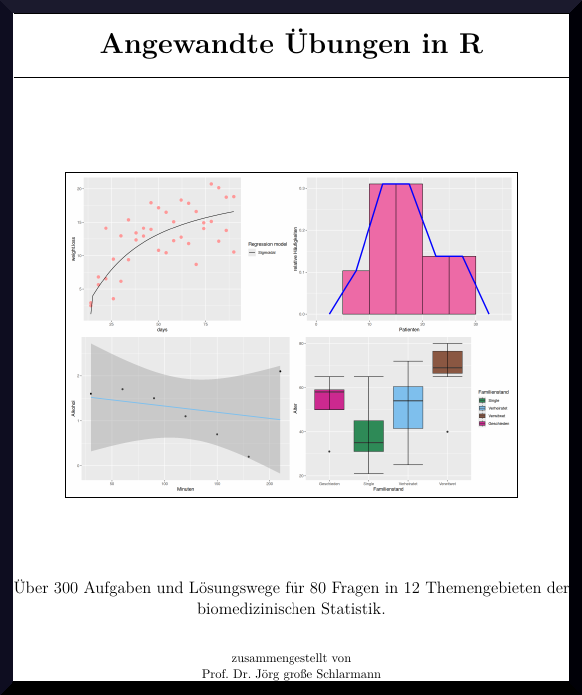
\includegraphics[width=60mm,height=\textheight]{images/AngewandteUebungen.png}

}

\subcaption{große Schlarmann (2024a)}

\end{figure}%

\end{minipage}%

\end{figure*}%

\vfill

Prof.~Dr.~Jörg große Schlarmann

Hochschule Niederrhein, Krefeld

\href{mailto:joerg.grosseschlarmann@hs-niederrhein.de}{\nolinkurl{joerg.grosseschlarmann@hs-niederrhein.de}}

\url{https://www.produnis.de/R}




\end{document}
